--- /home/jesse/Analysis/FemtoAnalysis/LamKPublication/CERN/4_IRC/LamKPublication_BeforeAddressingIRC4Comments.tex
+++ /home/jesse/Analysis/FemtoAnalysis/LamKPublication/CERN/LamKPublication.tex
@@ -162,11 +162,11 @@
 With this method, two- (or many-) particle relative-momentum correlation functions are used to connect the final-state momentum distributions to the space--time distributions of particle emission at freeze-out.  
 The correlation functions are sensitive to quantum statistics, as well as strong and Coulomb final-state interactions (FSI).  
 Current femtoscopic studies are able to extract the size, shape, and orientation of the pair emission regions, as well as offer estimates of the total time to reach kinetic decoupling and the duration of particle emission~\cite{Lisa:2005dd, Lisa:2008gf}.
-The momentum and species dependence of femtoscopic measurements affirm the collective nature of the hot and dense matter created in heavy-ion collisions~\cite{Makhlin:1987gm, Akkelin:1995gh, Retiere:2003kf, Kisiel:2009eh}.
-Non-identical particle analyses additionally allow for the measurement of the space--time separation of the single particle source regions~\cite{Lednicky:1995vk, Voloshin:1997jh, Lednicky:2001qv, Retiere:2003kf}.
-
-In addition to characterizing the source region, femtoscopy allows one to extract nuclear scattering parameters, many of which are difficult or impossible to measure otherwise.  
-\LamK pairs, which only interact strong, are the subject of this analysis.
+The momentum and species dependence of femtoscopic measurements affirms the collective nature of the hot and dense matter created in heavy-ion collisions~\cite{Makhlin:1987gm, Akkelin:1995gh, Retiere:2003kf, Kisiel:2009eh}.
+Non-identical particle analyses additionally allow for the measurement of the space--time separation of the single particle source regions~\cite{Lednicky:1995vk, Voloshin:1997jh, Retiere:2003kf}.
+
+In addition to characterizing the source region, femtoscopy allows one to extract nuclear scattering parameters, many of which are difficult or impossible to measure otherwise.
+The subject of this analysis, \LamK pairs, interact only strongly; therefore, the studied femtoscopic signals are free from quantum statistical and Coulomb interaction effects.
 Calculations within Quantum Chromodynamics (QCD), the theory of the strong interaction, are notoriously difficult except in the regime of weak coupling, where perturbative methods may be applied. 
 The \LamK analysis presented offers low energy QCD measurements, which fall into the non-perturbative regime of QCD.
 Therefore, the \LamK analysis not only gives insight into the strong interaction, it will also help guide future QCD calculations.
@@ -336,8 +336,8 @@
 If a daughter is found to be shared among \Vz candidates in a given collection, only that with the smallest DCA to the primary vertex is kept.
 This procedure ensures unique single-particle collections before particle pairs are constructed; the elimination of shared daughters between the particles within each pair is described below in Sec.~\ref{PairConstruction}.
 The resulting invariant mass distributions for \Lam and \Ks collections in the 0--10\% centrality interval are shown in Fig.~\ref{fig:Purity}.
-For the purity estimations, the background signal is extracted by fitting the \minv distribution with a $4^{\mathrm{th}}$-order polynomial outside of the mass peak and assuming the distribution to continue smoothly beneath the mass peak.
-The \Lam and \ALam purities are estimated to be $P_{\Lambda(\overline{\Lambda})} \approx 95\%$, and that of the \Ks is $P_{\mathrm{K^{0}_{S}}} \approx 98\%$.
+For the purity estimations, the background signal is extracted by fitting the \minv distribution with a fourth-order polynomial outside of the mass peak and assuming the distribution to continue smoothly beneath the mass peak.
+The \Lam and \ALam purities are estimated to be $P_{\Lambda(\overline{\Lambda})} \approx 96\%$, and that of the \Ks is $P_{\mathrm{K^{0}_{S}}} \approx 98\%$.
 
 \begin{table}[htbp]
  \centering 
@@ -345,7 +345,7 @@
   \renewcommand{\arraystretch}{1.05}
   \begin{tabular}{lc|c|l}
    \hlineB{3.0}  
-   \multicolumn{4}{c}{\Lam selection} \\
+   \multicolumn{4}{c}{\Lam [$\overline{\Lambda}$] selection} \\
    \hlineB{3.0}
    \multicolumn{3}{l|}{Transverse momentum $p_{\mathrm{T}}$} & $> 0.4$ GeV/\textit{c} \\
    \hline
@@ -471,7 +471,7 @@
     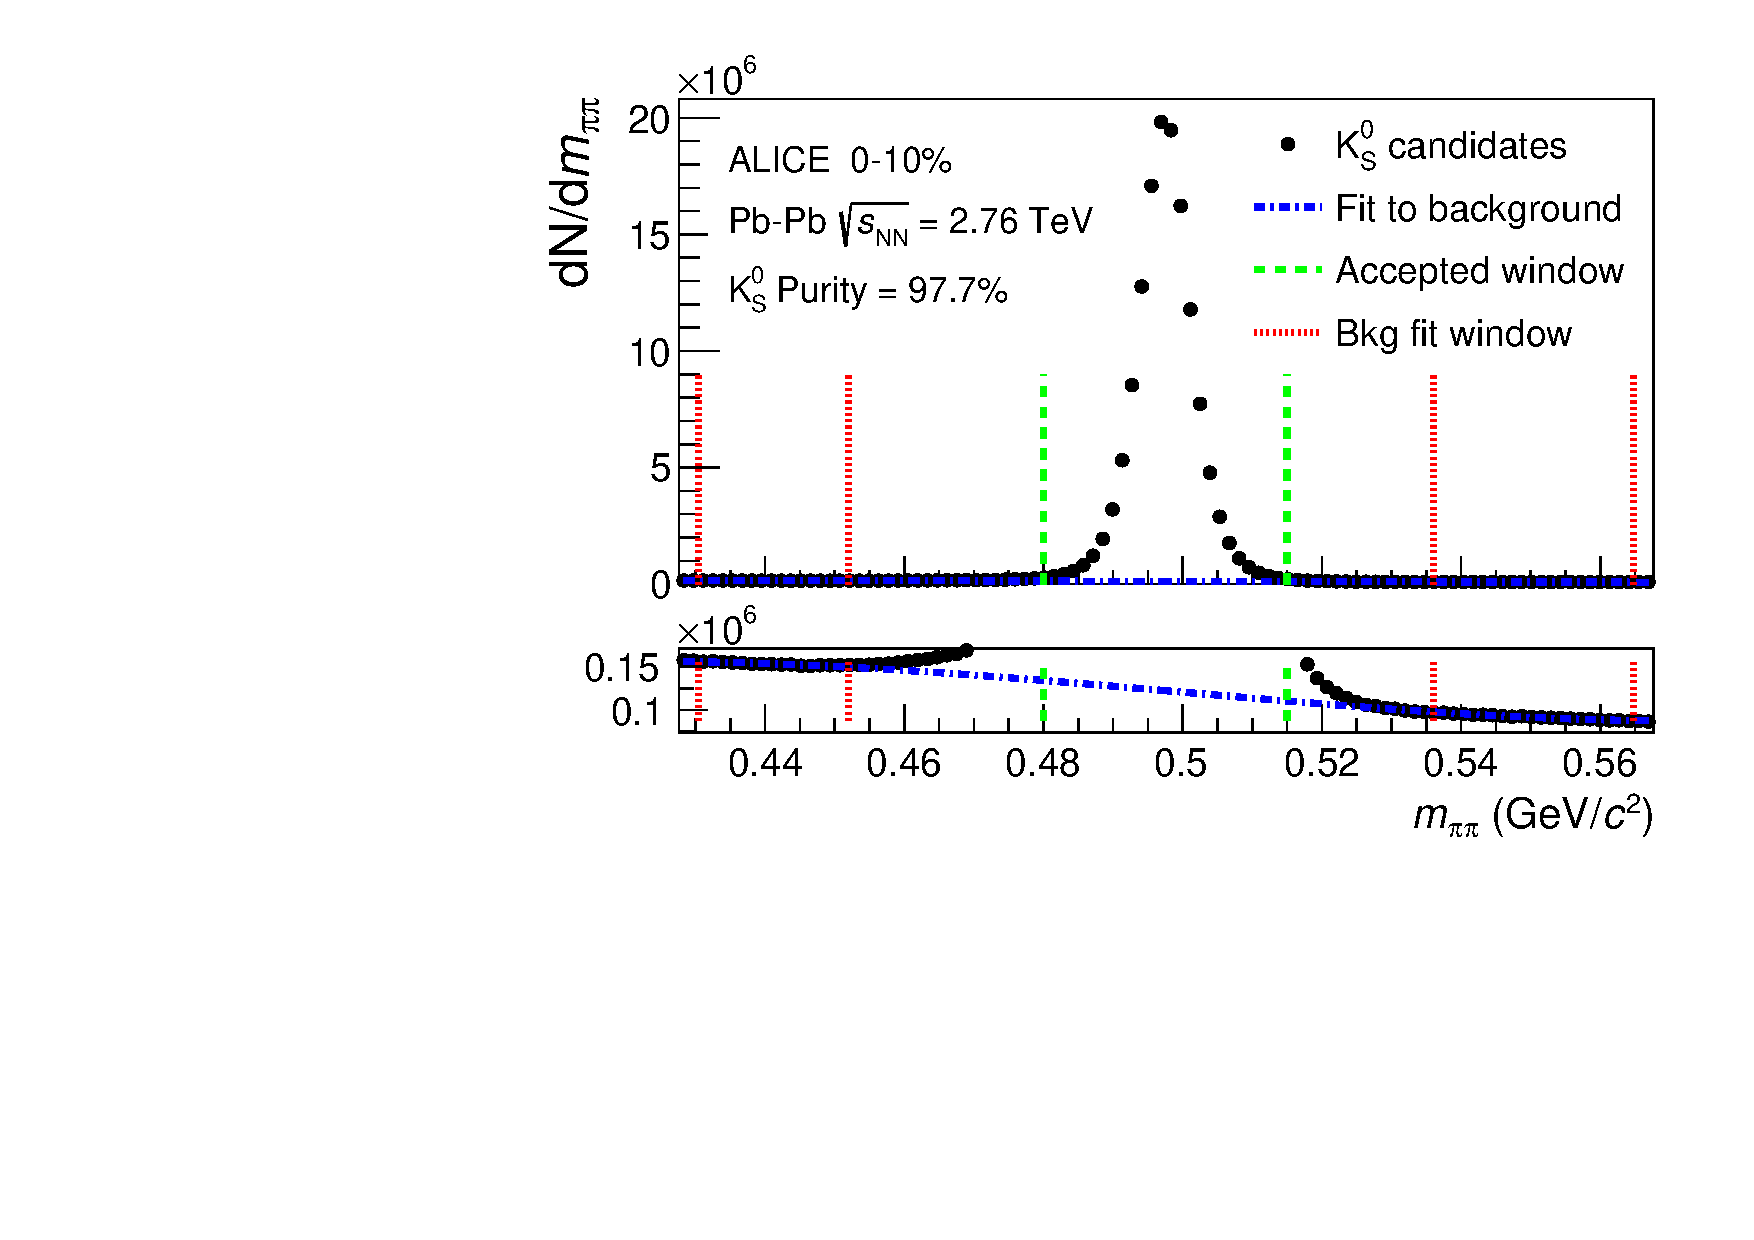
\includegraphics[width=0.49\linewidth]{/home/jesse/Analysis/FemtoAnalysis/LamKPublication/Figures/PDF/K0Purity_wPrintPurity_LamK0.pdf}}
   %%----overall caption----
   \caption{
-  (Color online) Invariant mass distributions in the 0--10\% centrality interval of (a) p$\uppi^{+}$ pairs showing the \Lam peak, and of (b) $\uppi^{+}\uppi^{-}$ pairs showing the \Ks peak, for \Vz candidates.  
+  (Color online) Invariant mass distributions in the 0--10\% centrality interval of (a) p$\uppi^{-}$ pairs showing the \Lam peak, and of (b) $\uppi^{+}\uppi^{-}$ pairs showing the \Ks peak, for \Vz candidates.  
   The bottom panels are zoomed to show the background with fit.  
   The vertical dashed (green) lines represent the selection restrictions used in the analyses, the vertical dotted (red) lines delineate the region over which the background was fit, and the dash-dotted (blue) line shows the background fit.
   }  
@@ -506,16 +506,16 @@
 %************************************************************************************************************************
 \subsection{Correlation function}
 \label{sec:CorrelationFunction}
-The two-particle correlation function for particles $a$ and $b$, $C_{ab}(\mathbf{p}_{a},\mathbf{p}_{b})$, is defined as the ratio of the probability of simultaneously measuring two particles with momenta $\mathbf{p}_{a}$ and $\mathbf{p}_{b}$, to the product of the single-particle probabilities.
-These probabilities are directly related to the covariant two-particle spectrum, $E_{a}E_{b}\frac{d^{6}N_{ab}}{d^{3}p_{a}d^{3}p_{b}}$, and the single-particle spectra, $E_{a(b)}\frac{d^{3}N_{a(b)}}{d^{3}p_{a(b)}}$, and the correlation function may be written
-\begin{equation}
-  C_{ab}(\mathbf{p}_{a},\mathbf{p}_{b}) = \frac{E_{a}E_{b}\frac{d^{6}N_{ab}}{d^{3}p_{a}d^{3}p_{b}}}{\big( E_{a}\frac{d^{3}N_{a}}{d^{3}p_{a}} \big) \big( E_{b}\frac{d^{3}N_{b}}{d^{3}p_{b}} \big)},
+The correlation function for particles $a$ and $b$, $C_{ab}(\mathbf{p}_{a},\mathbf{p}_{b})$, is defined as the ratio of the probability of simultaneously measuring two particles with momenta $\mathbf{p}_{a}$ and $\mathbf{p}_{b}$, to the product of the single-particle probabilities.
+These probabilities are directly related to the covariant two-particle spectrum, $E_{a}E_{b}\frac{\mathrm{d}^{6}N_{ab}}{\mathrm{d}^{3}p_{a}\mathrm{d}^{3}p_{b}}$, and the single-particle spectra, $E_{a(b)}\frac{\mathrm{d}^{3}N_{a(b)}}{\mathrm{d}^{3}p_{a(b)}}$, and the correlation function may be written
+\begin{equation}
+  C_{ab}(\mathbf{p}_{a},\mathbf{p}_{b}) = \frac{E_{a}E_{b}\frac{\mathrm{d}^{6}N_{ab}}{\mathrm{d}^{3}p_{a}\mathrm{d}^{3}p_{b}}}{\big( E_{a}\frac{\mathrm{d}^{3}N_{a}}{\mathrm{d}^{3}p_{a}} \big) \big( E_{b}\frac{\mathrm{d}^{3}N_{b}}{\mathrm{d}^{3}p_{b}} \big)},
 \label{eqn:CfRatioSpectra}
 \end{equation}
 where $N_{ab}$ is the yield of particle pairs, $E_{a(b)}$ is the energy, $p_{a(b)}$ is the three-momentum, and $N_{a(b)}$ is the yield of particles $a(b)$.
 Theoretically, the correlation function may be expressed as in the Koonin-Pratt equation~\cite{Koonin:1977fh, Pratt:1990zq},
 \begin{equation}
- C(\mathbf{k^{*}}) = \int S_{\mathbf{P}}(\mathbf{r^{*}})|\Psi_{\mathbf{k^{*}}}(\mathbf{r^{*}})|^{2}d^{3}\mathbf{r^{*}},
+ C(\mathbf{k^{*}}) = \int S_{\mathbf{P}}(\mathbf{r^{*}})|\Psi_{\mathbf{k^{*}}}(\mathbf{r^{*}})|^{2}\mathrm{d}^{3}r^{*},
 \label{eqn:KooninPrattEqn}
 \end{equation}
 where $\mathbf{k}^{*}$ is the relative momentum of the pair (defined as $\mathbf{k}^{*} = \frac{1}{2}|\mathbf{p}_{a}^{*}-\mathbf{p}_{b}^{*}|$, where $\mathbf{p}_{a}^{*}$ and $\mathbf{p}_{b}^{*}$ are the momenta of the two particles) in the pair rest frame (PRF, denoted with an asterisk $^{*}$), $\mathbf{r}^{*}$ is the relative separation in the same frame, $\mathbf{P}$ is the total pair momentum, $S_{\mathbf{P}}(\mathbf{r^{*}})$ is the pair source distribution, and $\Psi_{\mathbf{k^{*}}}(\mathbf{r^{*}})$ is the two-particle wave-function.
@@ -577,7 +577,7 @@
 Pairs in which at least one member originates from a particle decay (e.g., \LamKchP from $\Sigma^{0}$\KchP) carry information about the parent system.
 In effect, the correlation between the parents will be visible, although smeared out, in the daughters' signal.
 This is termed a residual correlation resulting from feed-down.  
-As described in the following, the main sources of residual correlations in the \LamK systems result from \Lam hyperons which have decayed from $\Sigma^{0}$, $\Xi^{0}$, and $\Xi^{-}$ parents. 
+As described in the following, the main sources of residual correlations in the \LamK systems result from \Lam hyperons which have been produced from $\Sigma^{0}$, $\Xi^{0}$, and $\Xi^{-}$ decays. 
 
 The measured correlation function is a combination of the genuine \LamK correlation with contributions from particle decays and impurities~\cite{Kisiel:2014mma},
 \begin{equation}
@@ -624,11 +624,11 @@
 The relevant reconstruction efficiencies are those of the daughters under study, not of the parent particles; e.g., when determining the contribution of the \XiKchP system to the \LamKchP correlation function, the reconstruction efficiency of the $\Xi^{-}$ is not relevant, but that of the secondary \Lam originating from a $\Xi^{-}$ decay is. 
 The reconstruction efficiencies ($RE_{ij}$) are estimated with HIJING simulations using GEANT3 to model particle transport through the detector.
 HIJING events are generated from a superposition of PYTHIA pp collisions, and lack the strangeness saturation of a fully thermalized medium.
-As a result, HIJING is unreliable in providing the yields needed for this analysis, and, instead, the yields are estimated with the THERMINATOR 2 simulation ($N_{ij}^{\scaleto{THERM}{3pt}}$).
-The number of \LamK pairs from source $ij$ is then estimated as the product of the yield with the associated reconstruction efficiency, $N_{ij} = N_{ij}^{\scaleto{THERM}{3pt}}RE_{ij}^{\scaleto{HIJING}{3pt}}$.
+As a result, HIJING is unreliable in providing the yields needed for this analysis, and, instead, the yields are estimated with the THERMINATOR 2 simulation ($N_{ij}^{\scaleto{\mathrm{THERM}}{4pt}}$).
+The number of \LamK pairs from source $ij$ is then estimated as the product of the yield with the associated reconstruction efficiency, $N_{ij} = N_{ij}^{\scaleto{\mathrm{THERM}}{4pt}}RE_{ij}^{\scaleto{\mathrm{HIJING}}{4pt}}$.
 Finally, the $\lambda_{ij}$ are estimated as
 \begin{equation}
-\lambda_{ij} = \frac{N_{ij}}{N_{Total}} = \frac{N_{ij}^{\scaleto{THERM}{3pt}}RE_{ij}^{\scaleto{HIJING}{3pt}}}{\sum\limits_{\alpha\beta} N_{\alpha\beta}^{\scaleto{THERM}{3pt}}RE_{\alpha\beta}^{\scaleto{HIJING}{3pt}}}.
+\lambda_{ij} = \frac{N_{ij}}{N_{\mathrm{Total}}} = \frac{N_{ij}^{\scaleto{\mathrm{THERM}}{4pt}}RE_{ij}^{\scaleto{\mathrm{HIJING}}{4pt}}}{\sum\limits_{\alpha\beta} N_{\alpha\beta}^{\scaleto{\mathrm{THERM}}{4pt}}RE_{\alpha\beta}^{\scaleto{\mathrm{HIJING}}{4pt}}}.
 \end{equation}
 
 
@@ -701,7 +701,7 @@
   C(k^{*}_{\mathrm{Rec}}) = \dfrac{\sum\limits_{k^{*}_{\mathrm{True}}}M_{k^{*}_{\mathrm{Rec}},k^{*}_{\mathrm{True}}}C(k^{*}_{\mathrm{True}})}{\sum\limits_{k^{*}_{\mathrm{True}}}M_{k^{*}_{\mathrm{Rec}},k^{*}_{\mathrm{True}}}},
 \label{eqn:MomResCorrection}
 \end{equation}
-where $M_{k^{*}_{\mathrm{Rec}},k^{*}_{\mathrm{True}}}$ is the response matrix, $C_{\mathrm{fit}}(k^{*}_{\mathrm{True}})$ is the fit as a function of \ktrue, and the denominator normalizes the result.
+where $M_{k^{*}_{\mathrm{Rec}},k^{*}_{\mathrm{True}}}$ is the response matrix, $C(k^{*}_{\mathrm{True}})$ is the correlation as a function of \ktrue, and the denominator normalizes the result.
 
 
 %************************************************************************************************************************
@@ -715,11 +715,11 @@
 
 The THERMINATOR 2 simulation has been shown to reproduce the background features in a $\uppi$K analysis~\cite{Kisiel:2017}. 
 Figure~\ref{fig:BgdswTHERM} shows the THERMINATOR 2 simulation together with experimental data.  
-The figure also shows a 6$^{\mathrm{th}}$-order polynomial fit to the simulation, as well as the fit polynomial scaled to match the data.
+The figure also shows a sixth-order polynomial fit to the simulation, as well as the fit polynomial scaled to match the data.
 Clearly, the THERMINATOR 2 simulation offers a good description of the non-femtoscopic backgrounds in the \LamK systems, and can be used in a quantitative fashion to help fit the data.
-More specifically, the non-femtoscopic backgrounds are modeled by 6$^{\mathrm{th}}$-order polynomial fits to THERMINATOR 2 simulation,
-\begin{equation}
-F_{\scaleto{THERM.\; Bgd}{6pt}}(k^{*}) = a{k^{*}}^{6}+ b{k^{*}}^{5} + c{k^{*}}^{4} + d{k^{*}}^{3} + e{k^{*}}^{2} + fk^{*} + g,
+More specifically, the non-femtoscopic backgrounds are modeled by sixth-order polynomial fits to THERMINATOR 2 simulation,
+\begin{equation}
+F_{\scaleto{\mathrm{THERM\; Bgd}}{6pt}}(k^{*}) = a{k^{*}}^{6}+ b{k^{*}}^{5} + c{k^{*}}^{4} + d{k^{*}}^{3} + e{k^{*}}^{2} + fk^{*} + g,
 \label{eqn:BgdPoly}
 \end{equation}
 where the linear term coefficient is fixed to zero ($f=0$), and one polynomial is fit for each centrality class and \LamK charge combination.
@@ -727,7 +727,7 @@
 Before fitting the signal region of the experimental data, the coefficients of each polynomial are fixed by fits to the THERMINATOR 2 background, shown in Fig.~\ref{fig:BgdswTHERM}.
 The extracted polynomial is adjusted to best describe the experimental data by introducing a scale factor and a vertical shift,
 \begin{equation}
-F_{\scaleto{Bgd}{6pt}}(k^{*}) = \alpha\cdot F_{\scaleto{THERM.\; Bgd}{6pt}}(k^{*}) + \beta,
+F_{\scaleto{\mathrm{Bgd}}{6pt}}(k^{*}) = \alpha\cdot F_{\scaleto{\mathrm{THERM\; Bgd}}{6pt}}(k^{*}) + \beta,
 \label{eqn:BgdScaleAndShift}
 \end{equation}
 where $\alpha$ and $\beta$ are determined by fitting to the data in the region $0.32 < k^{*} < 0.80$ GeV/$c$; all of the background parameters in Eq.~(\ref{eqn:BgdPoly}) and Eq.~(\ref{eqn:BgdScaleAndShift}) are fixed before fitting the low-\kstar signal region of the experimental correlation functions.
@@ -742,7 +742,7 @@
   (Color online) THERMINATOR 2 simulation (open squares) together with experimental data (closed circles).  
   Results are shown for \LamKchP (left), \LamKchM (middle), and \LamKs (right).
   Rows differentiate the different centrality intervals (0--10\% in the top, 10--30\% in the middle, and 30--50\% in the bottom).
-  A $6^{\mathrm{th}}$-order polynomial fit to the simulation is shown as a dashed curve.  
+  A sixth-order polynomial fit to the simulation is shown as a dashed curve.  
   This polynomial is scaled to match the experimental data and is drawn as a solid curve.
   }
   \label{fig:BgdswTHERM}
@@ -750,7 +750,7 @@
 
 
 An alternative approach to treating the non-femtoscopic background is to instead attempt to eliminate it.
-The background can be effectively reduced by forming the reference distribution ($B(k^{*})$) with the ``Stavinskiy method".
+The background can be effectively reduced by forming the reference distribution ($B(k^{*})$) with the ``Stavinskiy method"~\cite{Stavinskiy04, PhysRevD.82.052001} (see Appendix~\ref{App:StavMethod} for details).
 With this method, mixed-event pairs are not used for the reference distribution; instead, same-event pseudo-pairs, formed by rotating one particle in a real pair by 180$^\circ$ in the transverse plane, are used.  
 This rotation rids the pairs of any femtoscopic correlation, while maintaining correlations due to elliptic flow (and other suitably symmetric contributors).
 The flattening effect of the method on the \LamKchP correlation functions can be seen in the Appendix~\ref{App:StavMethod}.
@@ -978,11 +978,12 @@
 The use of this method in a three-dimensional analysis of two-pion correlations produced, in comparison to the event mixing results, an increase of 6\% for $R_{\mathrm{side}}$ at low-$k_{\mathrm{T}}$ and up to 4\% for $R_{\mathrm{out}}$ and $R_{\mathrm{long}}$~\cite{Aamodt:2011mr}.
 The purpose of using the Stavinskiy method in this \LamK analysis is to rid the correlation functions of the non-femtoscopic background.  
 More specifically, the intent is to handle background contributions from elliptic flow, and other sources having reflection symmetry in the transverse plane.  
-With the Stavinskiy method, mixed-event pairs are not used for the reference distribution; instead, same-event pseudo-pairs, formed by rotating one particle in a real pair by 180$^\circ$ in the transverse plane, are used.  
+With the Stavinskiy method, mixed-event pairs are not used for the reference distribution; instead, same-event pseudo-pairs, formed by rotating one particle in a real pair by 180$^\circ$ in the transverse plane, are used~\cite{PhysRevD.82.052001}.  
 This rotation rids the pairs of any femtoscopic correlation, while maintaining correlations due to elliptic flow (and other suitably symmetric contributors).
 Care needs to be taken in treating the pseudo-pairs exactly like the real pairs; e.g., the pseudo-pairs should be exposed to the same pair rejection procedures used in the analysis on the real pairs.
 The results of correctly implementing such a procedure are shown in Fig.~\ref{fig:StavCfs_Correct_LamKchP}.
 The figure demonstrates, for the \LamKchP system, that the Stavinskiy method is effective in flattening the correlation function in the region where no femtoscopic signal is expected.
+This procedure flattens the non-femtoscopic background equally well for the \LamKchM system, but is less effective for the \LamKs system.
 
 \begin{figure}[h!]
   \centering
@@ -1021,7 +1022,7 @@
 \end{equation} 
 In this case, the $\lambda$ parameter may be included as
 \begin{equation}
- C(\mathbf{k^{*}}) = (1 - \lambda) + \lambda\int S(\mathbf{r^{*}})|\Psi^{S}_{\mathbf{k^{*}}}(\mathbf{r^{*}})|^{2}d^{3}\mathbf{r^{*}}.
+ C(\mathbf{k^{*}}) = (1 - \lambda) + \lambda\int S(\mathbf{r^{*}})|\Psi^{S}_{\mathbf{k^{*}}}(\mathbf{r^{*}})|^{2}\mathrm{d}^{3}r^{*}.
 \label{eqn:GenCfEqnwLambda}
 \end{equation}
 To build a fit function for a system including both strong and Coulomb interactions two related options were considered. 
